\section{Related Work}

\subsection{Collecting System Calls}
There are several pieces of research to detect intrusions or unexpected behaviors
by collecting the system calls methods in runtime \cite{10.1007/978-3-319-24858-5_8,9307722,7809699,7796855}.
\textcite{10.1007/978-3-319-24858-5_8} proposed a real-time host-based intrusion
detection system in a container, which is based on system call monitoring. They use
the `strace' command to collect a behavior log to a system-call parser. Then use the
BoSC (Bag of System Calls) \cite{1495942} to classify is it a normal behavior in
the database.

The BoSC technique is a frequency-based detection tip. \textcite{1495942} defined
those distinct system calls in $\{c_1, c_2, \dots, c_n \}$, For all system call $s_i$
had been called in $c_i$ times. And they use Na\"ive Bayes classification to deduce if
it is unexpected behavior. Then the \citeauthor{10.1007/978-3-319-24858-5_8} give the false positive rate
of around 2\% in $O(S+n_k)$ epochs to the MySQL database \cite{10.1007/978-3-319-24858-5_8}.
\begin{itemize}
    \item Epoch Size ($S$): The total number of system calls in one epoch.
    \item $n_k$: It is the size of the database after epoch $k$.
\end{itemize}
However, the BoSC is running in user space, even though it is a background service running
on the same host kernel. It might have heavy constant time costs of copying data from
user to kernel and kernel to user by the `copy\_to\_user()' and `copy\_from\_user()' calls.\\

\textcite{7809699,7796855} takes a mathematical model to simulate the
smart moving target defense for Linux container resiliency. Considering an `ESCAPE' model
is the interaction between attackers and their target containers as a “predator searching
for a prey” search game. This search game has 3 modules: behavior monitoring, the
checkpoint/restore, and the live migration modules.
This model is running on the same host and the same attacking surface because they considered
the containers (prey) are running on the same machine with some migration probability.

They show the survival rate in \textcite{10.1007/978-3-319-24858-5_8} model for some
zero-day vulnerabilities in different types and numbers of machines.
\textcite{7809699,7796855} concluded that an IDS could detect and avoid mobile continually-growing
attacks efficiently by the `ESCAPE' model with collecting system calls.

\subsection{Fine-grained Permission Control}

The file system access control list (ACL) was defined in POSIX, which shares a naive and robust
permission model \cite{Grnbacher2003POSIXAC, 10.5555/3026877.3026930}. But after 20 years of
evolution, in the practical consideration of the Linux operating system design, it can be divided
into two permission control mechanisms: (\Rn{1}) POSIX ACL and (\Rn{2}) seccomp. Traditional
permission control is mostly controlled by ACL or similar. Many Linux secure modules (LSM) also
use ACLs for file access control\cite{Smalley2003ImplementingSA}. For example, SELinux and AppArmor
use such permission settings \cite{9184912, 217614, x11-SELinux, quteprints30563}.

\textcite{9184912} had proposed an architecture to enforce the access
control of the image's layers. Because the docker engine does not guarantee the layers could
not be modified by the host environment. Therefore, if we give a container privileged
permission, it could modify the layers of images. The research \cite{9184912} is using
the LSM's policy table to enforce the access control of the file system in the kernel.

\textcite{217614} proposed to separate the security namespace. Each container
can route its operation to different security namespaces for its "comment". Each
involved in the security namespace independently makes a security decision, and the
operation is allowed only if the policy engine allows it.

However, the policy engine has four types of policy conflicts: (\RN{1}) Parent-Child Conflict,
(\RN{2}) Global-Local Conflict, (\RN{3}) Lack of Authority, and  (\RN{4}) Environment does not
meet the expectation. The initial security namespace $\Phi$ is $\emptyset$. (\RN{1},
\RN{2}) will route the policy to $\Phi = \Sigma (\Phi \cap P_i), i \in \mathbb{N}, i < n$.
And the (\RN{3}, \RN{4}) is conflicted by the capabilities of that process. \textcite{217614}
give the capabilities a higher hierarchy than policy in the policy engine. Therefore
all of these conflicts will follow the capability first.

Android sandbox also uses ACL to control SELinux permissions for application registered users.
This is called in Android system UID-based discretionary access control (DAC).
And after Android 5.0, SELinux is provided to force the execution of DAC
\footnote{\url{https://source.android.com/security/app-sandbox}}.

\subsubsection{Capabilities}
\label{Capabilities}
Linux provides a more detailed permission control method on the file system, which is called
capability and was proposed by \citeauthor{6234805}. We can give archives some given capabilities
without giving hole root permissions when it executes specific system calls. Otherwise, it
must be a privileged process that can bypass all permission checks.

\subsection{Recently Exploited Vulnerabilities}
In this subsection, we will mention and review some `High' or `Critical' vulnerabilities
about kernel and containers in CVSS (Common Vulnerability Scoring System).
Because container is not a real virtual machine, it is an isolated process.

We ignore the CVE-2020-29389 series (CVE 306). Because those CVEs are not container or kernel's
vulnerabilities, those CVEs are issue of image defaults password. Despite those CVEs got 10.0 score,
those are small and unimportant vulnerabilities.

\subsubsection{Five Stages of Malware}
\label{Five_stage_of_malware}
We had been inspired by the quark engine\footnote{\url{https://quark-engine.readthedocs.io/en/latest/}},
which is an open-source malware scoring system for Android APK files. The quark
engine had been developed from the Taiwan Criminal Law's five stages:
(\Rn{1}) Determination, (\Rn{2}) Conspiracy, (\Rn{3}) Preparation, (\Rn{4}) Start, (\Rn{5}) Practice.\\

We also can use these five steps and category to give the malware stage to exploit the vulnerabilities.
(\Rn{1}) Base image landing, (\Rn{2}) Derived image landing, (\Rn{3}) User landing, (\Rn{4}) Kernel landing,
(\Rn{5}) Escaping. The escaping category is the worst case of container security, because we want a
container be a container, it must has zero leakage of capsulation.

\paragraph{Base image landing}
This is the most fundamentally basic assumption or guarantee of container security.
\textcite{inproceedings} proposed the BoSC technique must be $S = \{\emptyset\}$ in this step. By definition, for all
container $c$ is an image $I$ in execution, that is  $c = E(I)$. $E$ is a function to execute and
give container $c$ a description $\delta$ and a lifetime status $\lambda$. If we are using the docker environment, we can use the command:
\begin{codebash}
    docker inspect [NAME|ID...]
\end{codebash}
to get the description $\delta$ of the container. And we can use
\begin{codebash}
    docker ps [OPTIONS]
\end{codebash}
to get the lifetime status $\lambda$ of the container.
$$c=E(I)=\{\delta, \lambda\}$$
$\lambda \in \{$created, running, paused, stopped$\}$ statuses.

%\TODO{Graph}

It is called base image landed, if the BoSC technique $S \neq \{\emptyset\}$, which
might be injected some malicious item in the image. It is showed bellow.

%\TODO{Graph}

\paragraph{Derived image landing}
It is called derive image landing if some malicious items are inserted into the final layer,
while developers are inserting the application(s) and some dependencies into image layers,
It could be performed by a malicious base, dependencies, libraries, or binaries are inserted
into the filesystem. It is often in third-party unknown source image which is integrated
and republished by some crackers.

Those unknown source images could be replaced with the normal or official image by some hacks or overlays.
It looks fine when a user didn't check the image until who creates the instance of an image, that is container.
If the default application triggers the malicious part, it would give crackers a chance to take control of
the container. It would go to the next step user landing.

\paragraph{User landing}
It is the cracker landing into the container, no matter if it comes from a derived image or hacking from
the normal micro-application. Crackers might get a shell or execute some malicious binaries by
some injections or the other vulnerabilities.

In this step, the cracker could control the normal service to do the unexpected behaviors as
normal hacking scenarios. They can drop databases \cite{halfond2006classification} , practice
the local file inclusion \cite{hassan2018saisan, whitman2011principles}, etc.
Take an online judge in a container as an example: People could write some program, compile it, and execute it
on that machine. The cracker could write some malicious program or load some shellcode in those programs,
and give the operating system to execute. This is the user landing step.

If crackers could practice a remote code execution (RCE), they might get a sell and promote the privilege to
the super-user account in the container. They can do the same things as the host super-account except for
the capabilities in \ref{Capabilities}.

\paragraph{Kernel landing}

It is the hacker could hack the kernel
\cite{gaspar2006root, dam2018automatic, jimenez2016vulnerability, 10.1007/978-1-4020-8739-4_86}.
While the kernel copies data from the user and executes the user-provided malicious pattern
or the user exploits the kernel vulnerabilities, and lets that code executed in kernel mode, that is kernel landing.

It is kernel landing that we will introduce in the following subsubsection \ref{k_case}.

\paragraph{Escaping}

This is the most critical step of these five steps because this is the final utility given by the
container. Despite the kernel landing is almost control the whole machine, it is the last container
insecure issue of breaking the containers. There are three types of escaping: (\Rn{1}) Cgroups,
(\Rn{2}) Namespaces, (\Rn{3}) Capabilities.

(\Rn{1}) The cgroup escaping showed that \textcite{10.1145/3319535.3354227} break the
cgroups' limitation and affect the other container on the same host significantly, and gain
some extra resources from the host. (\Rn{2}) The namespace escaping shows in \ref{qemumachine}
demonstration paragraph.
The last one, (\Rn{3}) capability escaping can be overridden the capability after the kernel landing
and modify the `task struct' of the process in the kernel.

\subsubsection{Case Studies}
\label{k_case}

\paragraph{The Dirty CoW}
\textcite{8019988} showed the race condition and the mechanism of "Copy on
Write". "Copy on Write" is a resource-management technique used in computer programming
to efficiently implement a "duplicate" or "copy" operation on modifiable resources \cite{6394426}.
It is often inspired when `fork' or `mmap'.

\subparagraph{Mechanism}
Let's analyze the proof of concept (PoC) of the dirty CoW \cite{8019988} vulnerability
\footnote{\url{https://github.com/dirtycow/dirtycow.github.io/blob/master/dirtyc0w.c}}.
The key of inspiring this vulnerability is the mmaped memory space, which is mapped with
the PROT\_READ flag. The PROT\_READ flag declares that the page is read-only.
\lstinputlisting[language=C, linerange={87-89, 101-101}, firstnumber=87]{src/dirtyc0w.c}

It creates two threads, which would have a race condition of the mmaped memory space,
madviseThread and procselfmemThread.

\lstinputlisting[language=C, linerange={106-107}, firstnumber=106]{src/dirtyc0w.c}

In one thread, issuing a system call `madvise', would make the user thread gain the root
privilege to operate the protected page temporarily. And the flag MADV\_DONTNEED would
tell the kernel: "Do not expect to access it in the near future." Moreover,
this flag might not lead to immediate freeing of pages in the range. The kernel is free
to delay free the pages until an appropriate moment \footnote{\url{https://man7.org/linux/man-pages/man2/madvise.2.html}}.

\lstinputlisting[language=C, linerange={33-39,45-48}, firstnumber=33]{src/dirtyc0w.c}

In another thread, open its memory resource file. This file is a special file, which allows
the process to read its memory by itself.\\

Then, we move the printer of file descriptor of the memory resource file to the mmaped
space. And we try to write it. But the mmaped space is read-only. We expected that the
kernel would create a copy of this space and write the copy \cite{8001953}.\\
\lstinputlisting[language=C, linerange={50-53,61-63,67-71}, firstnumber=50]{src/dirtyc0w.c}

However, there is a problem! There is another thread that is racing this page with root
privilege. If the schedular context switches the madviseThread to procselfmemThread while
the adviseThread is calling the `madvise' system call, it would cause the
procselfmemThread to gain the root privilege from madviseThread to control the mmaped file.

\subparagraph{Demo}\mbox{}\\
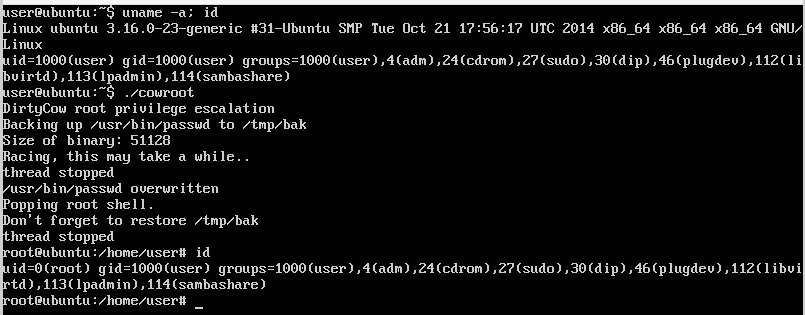
\includegraphics[width=.5\textwidth]{src/Screenshot_2021-12-26_05-14-58.png}
\label{qemumachine}

\paragraph{CVE-2016-8655 series}
We will introduce the series vulnerabilities related to CVE-2016-8655\footnote{
    \url{https://cve.mitre.org/cgi-bin/cvename.cgi?name=CVE-2016-8655}}, which are
CVE-2017-7308\footnote{\url{https://cve.mitre.org/cgi-bin/cvename.cgi?name=CVE-2017-7308}}
and CVE-2020-14386\footnote{\url{https://cve.mitre.org/cgi-bin/cvename.cgi?name=CVE-2020-14386}}.
These vulnerabilities are related to the bugs in net/packet/af\_packet.c in the kernel.
These series vulnerability is rely on the capability of CAP\_NET\_RAW\footnote{\url{https://linux.die.net/man/7/capabilities}},
which is a capability that can "use RAW and PACKET sockets and bind to
any address for transparent proxying" in Linux. And we had also introduced the Linux
capabilities at \ref{Capabilities}.

\subparagraph{CVE-2016-8655 and CVE-2017-7308} They are that there exists a race condition probability to
race the unauthorized data inside packet\_set\_ring() and packet\_setsockopt().
When we are using the PACKET\_RX\_RING option on the setsockopt(), and if the
version of the packet socket is TPACKET\_V3. Then we can race the init\_prb\_bdqc()
and swap(rb-$>$pg\_vec, pg\_vec) in packet\_set\_ring() with the spin lock rb\_queue-$>$lock.
However, when the socket was closed and called kfree() of the struct packet\_sock.
It causes a use-after-free on a kernel timer object that can be exploited
by various attacks on the SLAB allocator in setsockopt()
\footnote{\url{https://github.com/torvalds/linux/blob/f6fb8f100b807378fda19e83e5ac6828b638603a/net/packet/af\_packet.c\#L3690}}
\footnote{\url{https://googleprojectzero.blogspot.com/2017/05/exploiting-linux-kernel-via-packet.html}}.

They are critical vulnerabilities that can impact all Linux distributions' kernels being
built from 2011 to 2016. We can use these vulnerabilities to land on the kernel in
containers, such that the container would be controlled by crackers.

\subparagraph{CVE-2020-14386} It is a combination of CVE-2016-8655 and CVE-2017-7308 above.
Despite people patch those vulnerabilities, there exist an arithmetic overflow, because
the variable of netoff is an offset of ethernet header which is only stored in an unsigned
short. Crackers can produce an arithmetic overflow when they have the CAP\_NET\_RAW capability,
which value must be smaller than INT\_MAX, but receive a larger value than the size of a
block and write beyond the bounds of a frame buffer\footnote{\url{https://www.openwall.com/lists/oss-security/2020/09/03/3}}.

Or Cohen submitted the patch\footnote{\url{https://github.com/torvalds/linux/commit/acf69c946233259ab4d64f8869d4037a198c7f06}}
to fix this CVE-2020-14386, and this patch is integrated into Linux 5.8. This vulnerability
is also a kernel-level bug that can gain root privileges from unprivileged processes.
Therefore, a cracker could use this vulnerability to get the privilege to escape from containers.

People notice that it is impossible to do any protection if the kernel has vulnerabilities
that the container has the capability to ask the kernel to execute malicious code directly. Despite
they make the kernel up-to-date, there also have some probability that crackers could exploit
the kernel and brake the container. Because, containers are just isolated processes, they
are using the shared kernel as the host. When this bug is published, google's gVisor said
"Hey, we are immunity to this vulnerability." \footnote{\url{https://cloud.google.com/blog/products/containers-kubernetes/how-gvisor-protects-google-cloud-services-from-cve-2020-14386}}
Because the gVisor implements its own network stack in its gVisor sandbox by the go language.
They do not ask for these supports from the kernel.

\paragraph{RunC exploits}

This sub-subsubsection would introduce some exploits for the runC engine.
RunC is an abbreviation of "run container", which is an instance of the host OS's process and the
parent process of a container environment.
% https://docs.google.com/presentation/d/1OpsvPvA82HJjHN3Vm2oVrqca1FCfn0PAfxGZ2w_ZZgc/edit
% https://developers.redhat.com/blog/2018/02/22/container-terminology-practical-introduction#container_orchestration

\subparagraph{CVE-2019-5736}
This is an attack that modifies the driver from the immutable layer. This attack
overwrites runC's binary file such that another program would be launched via runC to
reentrant this runC's container. It is quite dangerous to use binary files directly
from the file system because each container's file system is referenced from the instance
of the image file. Despite that an image is immutable, a container is mutable except for ACL controls.

In order to solve the problem of such duplication, a memfd is used instead, and
then runC is the driver of the container \footnote{\url{https://github.com/opencontainers/runc/commit/0a8e4117e7f715d5fbeef398405813ce8e88558b}}.
In this way, if a hacker rewrites the driver with any permission, at most it will only modify
the volatile program in memory. It will not overwrite the original immutable layer.
The user reentrants this container the next time, the hacker-modified runC will
not be triggered.

\subparagraph{CVE-2021-30465}
% https://blog.champtar.fr/runc-symlink-CVE-2021-30465/
% https://github.com/opencontainers/runc/security/advisories/GHSA-c3xm-pvg7-gh7r
There is a race condition between checking the filesystem while the container is
starting and actually mounting it into the container. The original researcher found
this race condition problem on k8s \footnote{\url{https://blog.champtar.fr/runc-symlink-CVE-2021-30465/}}.
However, there is a bug that we have full control permission over the file that
is mounted in a container. Therefore the researcher creates 20 containers to race a shared
directory that placed a symbolic link to the container's outside.

\lstinputlisting[language=C, linerange={10-38}, firstnumber=10]{src/race.c}

We can see the PoC code as above.

\subsection{A Minimal Cross-platform Container in Linux}
A kernel-level virtualization, which is so-called a container, is constructed by two
features: hardware limitation, namespace limitation. We can use the `mount' with a tag of
cgroup system call in Linux to create an association set of parameters for hierarchy
subsystems \footnote{\url{https://www.kernel.org/doc/html/latest/admin-guide/cgroup-v1/cgroups.html}}.
We use the `clone' or `unshare' to manipulate the task\_struct in the kernel.

We give the container all the hardware usage to our mini-container, and execute from a thread of
function 'run'.
\lstinputlisting[language=C, linerange={45-49}, firstnumber=45]{src/lc/cont.c}
We use the clone \footnote{\url{https://man7.org/linux/man-pages/man2/clone.2.html}} with
CLONE\_NEWNS flag to start in a new mount namespace, initialing with a copy of the
namespace of the parent. Then, we use chroot to limit the child process's root directory
to our "rootfs".
\lstinputlisting[language=C, linerange={18-30}, firstnumber=18]{src/lc/cont.c}
So we start the first program in the container, which would be executed in the
our-designed container, which is shown in figure \ref{lc}.
    {
        \begin{figure}
            \centering
            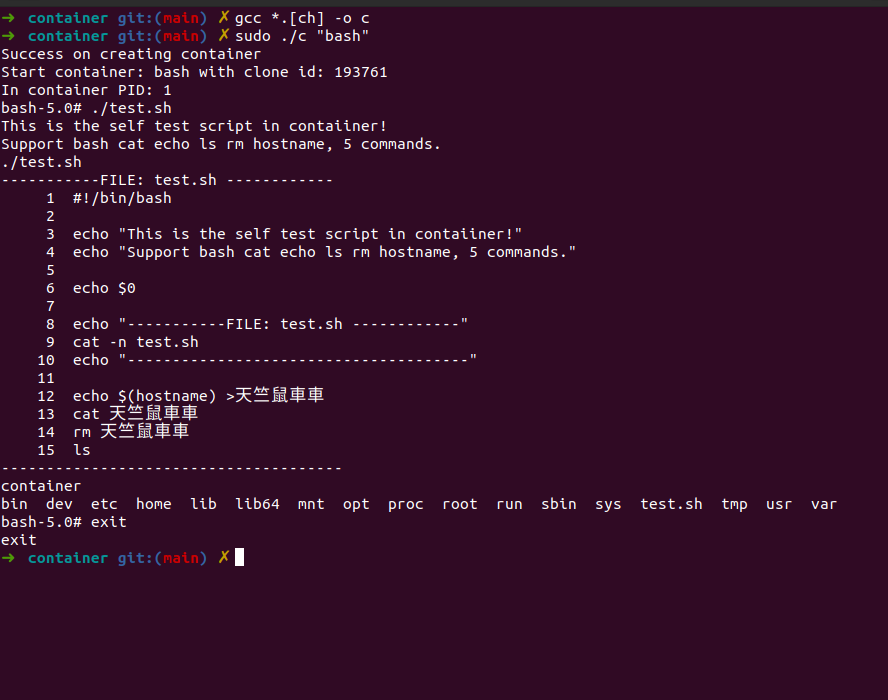
\includegraphics[width=.5\textwidth]{src/cur_cont.png}
            \blodcaption{A Minimal Cross-platform Container in Linux}
            \label{lc}
        \end{figure}
    }
\lstinputlisting[language=C, linerange={32-43}, firstnumber=32]{src/lc/cont.c}

But there is a problem here. That is the program could not be loaded normally while
the kernel tries to load the dynamic libraries into memory, which depends on the
binary program. This is the reason why we need an immutable base file system layer to
support the container image.

Suppose we build the minimal container on a self machine, we can assume the CPU architecture
is the same. Therefore we can copy the dependencies to "rootfs" directly.

\lstinputlisting[language=sh, linerange={10-46}, firstnumber=10]{src/lc/build.sh}

\subsection{Virtual Environment Performance Benchmark}
There is a trend of applications are developed or deployed into microservice in a virtual
environment since 2008. And the performance benchmark of applications in the virtual
environment becomes more and more critical.

Therefore, there are many pieces of research shows how to evaluate the performance when
using containers or the other virtual infrastructures\cite{7371699,KOZHIRBAYEV2017175,7095802,234857}.
They are comparing the throughput, latency, and QoS for memory IO, or cryptography
algorithms calculating costs.\\

\textcite{234857} showed the gVisor costs: $2.2\times$ system call overhead,
$2.5\times$ memory allocation latency, and $216\times$ \textbf{slower} than raw system on
complex file opening. And \textcite{KOZHIRBAYEV2017175} showed that I/O times have more
disadvantages of latency and throughput, which is compared to container and native machines.
